
\documentclass[11pt,a4paper,oneside]{report}
\usepackage{mathpazo} 
\linespread{1.05}        
\usepackage[scaled]{helvet} 
\usepackage{courier} 

\normalfont
\usepackage[T1]{fontenc}
\usepackage[footnotesize]{caption}


\linespread{1.05}         

\parskip 7.2pt

\usepackage{setspace}
\onehalfspacing

\usepackage{framed}

\usepackage{pdfsync}

\setlength{\parindent}{0in} 


\usepackage[pdftex]{graphicx}

\usepackage{amsmath}
\usepackage{amssymb,amsfonts,textcomp}


\usepackage{color}
\definecolor{gray09}{rgb}{0.9,0.9,0.9}  
\definecolor{red}{rgb}{1,0,0}
\definecolor{blue}{rgb}{0,0,1}
\definecolor{lightblue}{rgb}{0,0.8,1}
\definecolor{Dark}{gray}{.2}
\definecolor{Medium}{gray}{.6}
\definecolor{Light}{gray}{.8}
\definecolor{shadecolor}{rgb}{0.9, 0.9, 1}


\usepackage{epstopdf}

\usepackage{natbib}
\bibpunct{(}{)}{;}{a}{,}{,}

\usepackage{hyperref}
\hypersetup{colorlinks=true, 
	citecolor=blue, 
	linkcolor=black, 
	urlcolor=black}

\usepackage{pdfpages}


\usepackage{supertabular}
\usepackage{array}
\usepackage{supertabular}
\usepackage{hhline}


\usepackage{float}
\usepackage{subfig}

\usepackage{fancyhdr}
\setlength{\headheight}{15.2pt}
\pagestyle{fancyplain}
\renewcommand{\chaptermark}[1]{\markboth{#1}{}}
\renewcommand{\sectionmark}[1]{\markright{\thesection\ #1}{}}
 
\lhead{\fancyplain{}{\textit{BIAS2017}}}
\chead{}
\rhead{\fancyplain{}{\textit{\rightmark}}}
\lfoot{}
\cfoot{\fancyplain{}{\thepage}}
\rfoot{}



\newenvironment{indentexercise}[1]
{{\setlength{\leftmargin}{2em}}
\textbf{Exercise \thesubsection-#1}
\begin{list}{}
	\item
}
{\end{list}}

\newenvironment{indentFiji}
{\begin{list}{}
         {\setlength{\leftmargin}{1em}}
         \item[]
}
{\end{list}}

\newenvironment{indentCom}
{\begin{list}{}
         {\setlength{\leftmargin}{1em}}
         \item[]
}
{\end{list}}

\newcommand{\ijmenu}[1]{\texttt{\small#1}}

\newcommand{\ilcom}[1]{\texttt{\small#1}}

 \newcommand{\tab}{\hspace*{3em}}

\newcommand{\HRule}{\rule{\linewidth}{0.5mm}}

\usepackage{textcomp}
\newcommand*{\micro}{\textmu}



\usepackage{listings}
\lstset{ 
basicstyle=\small\ttfamily, 
numbers=left,                   
numberstyle=\footnotesize,      
stepnumber=1,                   
numbersep=5pt,                  
backgroundcolor=\color{gray09},  
keywordstyle=\color{red}, 	
showspaces=false,               
showstringspaces=false,         
showtabs=false,                 
tabsize=2,                      
captionpos=b,                   
breaklines=true,                
title=\lstname,                 
escapeinside={\%*}{*)},         
morekeywords={*,...},            
morecomment=[l]{//},
morecomment=[s]{/*}{*/},
morestring=[b]",
}



\newcommand*{\titleTH}{\begingroup
\raggedleft
\textsc{\textbf{\Large{NEUBIAS}}}
\HRule\\
\vspace*{\baselineskip}

\hfill \textsc{\large Authors:}\\
[0.3\baselineskip]
\hfill {\Large Kota Miura}\\
{\small EMBL Heidelberg, NIBB Okazaki}\\
\vfill

{\textcolor{Medium}{\Large ImageJ Macro Language}}\\
[\baselineskip]
{\Large - Part I -}\\
[2\baselineskip]

{\bfseries NEUBIAS Textbook Series}\\
\textbf{Continuous Release}

\vfill

\hfill \textsc{Reviewers / Teachers:}\\
[0.3\baselineskip]
\hfill {\large Kristine Schauer}\\
\hfill {\small Institut Curie Paris}\\
[0.3\baselineskip]
\hfill {\large Christian Tischer}\\
\hfill {\small EMBL Heidelberg}\\
[0.3\baselineskip]
\hfill {\large Chong Zhang}\\
\hfill {\small SIMBioSys, Universitat Pompeu Fabra}\\
\HRule\\

{\small \hfill\textcolor{Medium}{ Compiled on: \today }}
\endgroup}

\begin{document}

\date{\today}

\pagestyle{empty}
\titleTH
\clearpage
\pagestyle{fancyplain}

\begingroup
\hypersetup{linkcolor=blue}
\tableofcontents
\endgroup

\clearpage

\setcounter{chapter}{2}


\section{Aim: Why do we write ImageJ macro?}
  
The aim of this small chapter is to teach the basics of how to automate image processing and analysis using ImageJ macro language. Why do we write ImageJ macro? We write macros to decrease our workloads in image processing: less clicking and less repetitive procedures. 
   
\section{Introduction}
  

\subsection{ImageJ macro makes your life easier}

To customize functions in ImageJ, a typical way is to write a Java plugin that directly accesses the application interface of ImageJ. 
This is a powerful method for customizing your own tool but in many cases is a bit too much for small tasks we often encounter in biological research projects. Compared to the Java programming, ImageJ macro is much easier to access and to quickly solve problems.

A typical usage is to automate repetitive tasks with hundreds of times of mouse clicking. Clicking could range from menu selections to inspection of single pixel value. By writing a macro, we could save such exhausting job to a single execution of a macro file, which is a text file with a sequence of image processing commands. As ImageJ macro functions are directly mirroring the GUI menu items, one could intuitively learn how to write one's own macro even without much experiences in programming.

Another important aspect of writing a macro is its role as a documentation: as the processing becomes complex, we easily forget the steps and details of the procedures and the values of parameters that were used for that task. Even if your job is not a repetitive one, a macro written for a task becomes a valuable record of what was done to the image, and ensures the \textbf{reproducibility} of your image analysis.  

\subsection{Other ways to Customize ImageJ}

This and the next section explain the general capability of extending ImageJ by programming. If you are not interested in general aspects, you could skip these sections.  

ImageJ could be extended by writing a Java plugin. Though you need to know or learn the Java programming,  this capability affords almost infinite possibilities;  you could write any kind of processing / analysis functions you could imagine. Compared to the plugin development by Java, ImageJ Macro language is much easier and lighter but has some limitations. It might be worth mentioning here what would be the limitations. 

\begin{enumerate}
\item If you need to process large images or stacks with many steps, 
you might recognize that it is slow. Some benchmarks indicate that a plugin would be about 40 times faster than a macro. 

\item Macro cannot be used as a library
  \footnote{It is possible to write a macro in a library fashion using the function \ilcom{eval} and use it from another macro, 
but this is not as robust and as clear as it is in Java, which is a language designed to be so.}. 
In Java, once a class is written, this could be used later again for another class. 

\item Macro is not efficient in implementing real-time interactive input 
during when the macro function is executed; 
\textit{e.g.} If you want to design a program that requires real-time user input 
to select a ROI interactively.  
Macro could only do such interactive tasks by closely related macro set with each macro doing each step of interaction. 

\item Macro is tightly coupled to GUI (Image Window), so that when you want to process images without showing them on desktop, macros are not really an optimal solution.
\end{enumerate}

If you become unsatisfied with these limitations, 
learning more complicated but more flexible Java plugin development is recommended. 


\subsection{Comparison with Other scripting languages}

Besides ImageJ macro, there are several scripting languages that
could be used for programming with ImageJ. The bare ImageJ supports Javascript (Rhino). Recent versions of ImageJ (> 1.47m,  since 6 March 2013), Jython became included in the menu as well. 
In the Fiji distribution, you could use the following languages off the shelf
\footnote{As of June, 2015}
:

\begin{itemize}
 \item Javascript
 \item BeanShell
 \item Jython (Java implemented Python)
 \item JRuby (Java implemented Ruby)
 \item Clojure
 \item Groovy
 \end{itemize}

If you set up an environment by yourself, other languages such as Scala can be used. 
Compared to the ImageJ macro language, all these languages are more general scripting languages. 

There are pros and cons. Pros of using the ImageJ Macro compared to these scripting languages are: 
\begin{itemize}
\item Easy to learn. 
ImageJ macro build-in functions are mirrors of ImageJ menu, so scripting is intuitive if you know ImageJ already. 
Macro recorder is a handy tool for finding out the macro function you need. 

\item A significant hurdle for coding with general scripting languages is that one must know the 
\textbf{ImageJ Java API} well, meaning that you basically have to know 
fundamentals of Java programming language for using these scripting languages. 

\item You could have multiple macros in one file (called 'Macro-set"). 
This is useful for packaging complex processing tasks.

\end{itemize}

Thus, ImageJ macro language is the easiest way to access the scripting
capability of ImageJ.

There are several disadvantages of ImageJ macro compared to other
scripting languages. First is its generality. Since others are based on major scripting languages, you do not need to learn a lot if you know one of them already. For example, if you know Python already, 
it should be easy for you to start writing codes in Jython (note: but you also need to know about Java). 

The second disadvantage of ImageJ macro is its extendability.
Codes you wrote could only be recycled by copying and pasting
\footnote{One could also use getArgument() and File related functions to pass
arguments from a macro file to the other, but ImageJ macro is not designed to
construct a library of functions.}.
With other scripting languages, once you write a code, it could be used from other programs
\footnote{ Calling other Javascript file from another Javascript file had been difficult but became easily possible in the Fiji distribution from March 2012.}.

Lastly, although ImageJ Macro processes with a speed comparable to
Javascript and Jython, it is slow compared to Clojure and Scala. 

\subsection{How to learn Macro programming}

In this course, you will encounter many example codes. 
You will write example codes using your own computer and run those macros. 
Modifying these examples by yourself is an important learning process as in most
cases, that is the way to acquire programming literacy. There are many excellent macro codes you could find in Internet, which could be used as starting points for writing your code\footnote{200+ macros are available in ImageJ web site. 
\href{http://rsb.info.nih.gov/ij/macros/}{http://rsb.info.nih.gov/ij/macros/}}.

\subsection{Summary}
ImageJ Macro radically decreases your work load and is a practical way to keep your image analysis workflow in text file. Less workload provides more time for us to analyze details of image data. 
The potential of macro is similar to other scripting languages and Java Plugins, all adding capability to customize your image analysis. For coding interactive procedures PlugIn works better than macro. Macro cannot be used as a library.  
Image processing by macro is slower than that by Java written plugins. 
 
\newpage

\section{Tools}
\label{sec:tools}
 
\begin{itemize}
  \item ImageJ (Fiji distribution).
  \begin{itemize}
    \item \url{http://fiji.sc}
    \item We use the Fiji distribution since it has ScriptEditor, a handy editor for writing macro. 
  \end{itemize}
  \item ImageJ Plugin: EMBL\_sampleimages-1.0.0.jar
  \begin{itemize}
     \item This plugin allows you to download sample image stacks. All the image files mentioned in this ``ImageJ Macro Language'' module could be opened by selecting the file name in \ijmenu{[EMBL > Sample Images >]}. Specified image file in the EMBL web server is then downlaoded and appears on your desktop.
    \item This plugin could be installed in one of the two following ways:
    \item First, using the ``Update Sites'' function in Fiji. Add ``CMCI-EMBL'' to your update sites by the updater interface that could be acceded via \ijmenu{[Help > Update Fiji]}. This ``update site'' function is pretty new in Fiji and usable with the latest Fiji version (2014\~)        
    \item Second, download the plugin from \url{http://cmci.embl.de/downloads/coursemodules}. 
  \end{itemize}
\end{itemize}
 
\newpage

\section{Basics}
\label{sec:ImageJMacroBasics}

  \subsection{``Hello World!''}
We first try writing a simple macro that prints ''Hello World!'' in the log window of ImageJ. For this, we use a text editor that comes with Fiji, called ``script editor''. 
It has some convenient features such as automatic coloring of macro functions {In programming world, we call this feature ``syntax highlighter''}. 

If you are not using Fiji and using native ImageJ, it's no problem as there is a simpler but perfectly working text editor. Macros we write in this textbook works exactly same in both editors. If you want to use the simple text editor for the following tutorial, its usage is explained after the explanation about Fiji edior (page \pageref{part:nativeeditor}).   

Let's open the ``script editor'' 
by \ijmenu{[File -> New -> Script]}. It should look like figure \ref{fig_ScriptEditor}.
There should be a blank text field where you write your macro. Since the editor allows you to write different scripting languages as well, you should first select the language you are going to use.  
From script editor's own menu, select \ijmenu{[Language -> IJ1 Macro]}. 

Then, write your first macro as shown below (see also figure \ref{fig_ScriptEditor}). \\
\begin{lstlisting}[numbers=none]
print("Hello World!");
\end{lstlisting}

Don't ignore quotation marks, parenthesis and the semi-colon! 
Syntax highlighter offers automatic coloring of ImageJ functions, because you selected the language "IJ macro" in above. It increases the readability of codes. 

Then in the bottom-left corner of the script editor, there is a button labeled "Run". Clicking this, you will see that a log window is created (if it is already there, then it will have a new line) printing "Hello World!" (Figure \ref{fig_HelloWorldLog}). Another way to run the macro is via Script Editor menu,  \ijmenu{[Run -> Run]} . You could use Ctrl-R (Windows) or Command-R (OSX) as well.  

Later when you want to start writing another macro, you could just create a new tab by \ijmenu{[File > New]} and then select \ijmenu{[Language -> ImageJ Macro]} again.

\begin{figure}[hbtp]
\begin{center}
\includegraphics[scale=1.0]{fig/editor_helloworld_singleline.png}
\caption{Script Editor of the Fiji distribution} \label{fig_ScriptEditor}
\end{center}
\end{figure}

\begin{figure}[hbtp]
\begin{center}
\includegraphics[scale=1.0]{fig/helloworld_logwindow.png}
\caption{Hello World Output} \label{fig_HelloWorldLog}
\end{center}
\end{figure}


\subsubsection{Simple Text Editor in native ImageJ}
\label{part:nativeeditor}

If you are using native imageJ, the the macro editor launches by selecting \ijmenu{[PlugIns -> New -> Macro]} from the menu (\ref{fig_MacroEditor}). 
Please write the following line in the editor. 
\begin{lstlisting}[numbers=none]
print("Hello World!");
\end{lstlisting}
From the menu of the macro editor (in OSX, the menu switches to the editors own menu when the editor window is active), select [Macros > Run Macro]. You should then see "Hello World!" printed in the log window. 

The macro editor has simple debugger function, which is not present in Fiji script editor. Debugger assists you to correct mistakes in the code. ImageJ Macro can be written in any text editor such as "Notepad" in Windows but of course there is no debugger function available in this case.

\begin{figure}[htbp]
\begin{center}
\includegraphics[scale=0.6]{fig/editor_helloworld_IJ_simple.png}
\caption{Macro Editor of ImageJ} \label{fig_MacroEditor}
\end{center}
\end{figure}


\subsubsection{Anatomy of ``Hello World!''}

Let's see more details of what the single line code we wrote is doing.

\ilcom{print()} is a build-in macro function that requests ImageJ to take the content within the parenthesis and print that out in the "Log" window. This content, which we genearlly call the \textit{argument} of the function, is an input value given to the function. The output of this function is the printed text in the Log window. Note that when a text is given as an argument, it must be surrounded by double quotes ("").
 
Where do we get information as such for other macro functions? The best reference for ImageJ macro functions is in the ImageJ web site
\footnote{\url{http://rsbweb.nih.gov/ij/developer/macro/functions.html}}. 
For example, you could find definition of \ilcom{print("")} function on the web site as quoted below:\\
\begin{indentCom}
\fbox{
\parbox[b][20em][c]{0.80\textwidth}{
\textbf{print(string)}\\
Outputs a string to the "Log" window. Numeric arguments are automatically converted to strings. 
The print() function accepts multiple arguments. For example, you can use print(x,y,width, height) 
instead of print(x+" "+y+" "+width+" "+height). 
If the first argument is a file handle returned by File.open(path), 
then the second is saved in the referred file (see SaveTextFileDemo).

Numeric expressions are automatically converted to strings using four decimal places, 
or use the \ilcom{d2s} function to specify the decimal places. 
For example, print(2/3) outputs "0.6667" but print(d2s(2/3,1)) outputs "0.7".

\dots
}
}
\end{indentCom}

As \ilcom{print} can do many things, its explanation is extraordinary long, but by carefully reading it, you will save time afterwards by the knowledge of wide spectrum of things that the \ilcom{print} function can do e.g. directly save text as a file. 


Macro can be saved as a file.
In the editor, do \ijmenu{[File -> Save]}. Just save the file wherever you want in your file system. When you want to use the macro again, load the macro by \ijmenu{[File > Open]}.

\begin{indentexercise}{1}
\item Add another line \texttt{"print("\textbackslash{}\textbackslash{}Clear");"} 
before the first line (below, code 1.51. don't forget the semi-colon at the end!). 
\item 
\begin{lstlisting}
//code 1.5
print("\\Clear");
print("Hello World!");


\end{lstlisting}
\textbf{sourcecode}: \href{http://www.example.com/contents}{code/code01\_51.ijm}
Then test also another macro when you put the same line after "Hello World!". 
What happened? Any difference in the behavior? 
\item 
\begin{lstlisting}
//Code 1.76
print("Hello World!");
print("\\Clear");
\end{lstlisting}
\textbf{sourcecode}: \href{http://www.example.com/contents}{code/code01\_76.ijm}
\item \textbf{Answer}: The first code prints "Hello World!", while the second code prints nothing. This is becaise \ilcom{print("\textbackslash{}\textbackslash{}Clear")} is a command that clears the Log window. In the first code, ``Hello World'' is printed after the window clearing, and in the second case the Log window is wiped out right after the printing of ``Hello World''. Effectively it looks like nothing has happened.  
\end{indentexercise}

\begin{indentexercise}{2}
\item Try modifying the third line in code 1.51
and check that the modified text will be printed in the "Log" window. \\
\end{indentexercise}

\begin{indentexercise}{3}
\item Multiple macros can exist in a single file. We call this \textbf{"macro sets"}. To distinguish each macro, each they each should have a specific name. For this, each macro should start with a special word ``macro'' followed by the name of the macro, and then a pair of curly braces to encapsulate its macro functions. See the code below (code01\_8.ijm).  

Modify the code you already wrote in the script editor to wrap it inside a pair of macro bounds, the curly braces (\ilcom{\{\}}).  Then copy and paste the same under the first macro. 
The second macro should be modified to have a different name. In the example shown in fig.
\ref{fig_MacroSetInMenu}, the second macro is named "print\_out2".

When macro is properly declared in this way, you could install the macro to have it as a menu item. To do so, in the editor menu select: 
\begin{indentFiji}
[Run -> Install Macro]).
\end{indentFiji}
In the main menu you should no be able to see the macro names under \ijmenu{[Plugins > Macros > ]}. See fig. \ref{fig_MacroInMenu}}
\end{indentexercise}

\begin{lstlisting}
macro "print_out" {
	print("Hello World!");
}

macro "print_out2" {
	print("Bye World!");
}

\end{lstlisting}
\textbf{sourcecode}: \href{http://www.example.com/contents}{code/code01\_8.ijm}


\begin{figure}[htbp]
\begin{center}
\includegraphics[scale=0.6]{fig/editor_MacroSet.png}
\caption{Macro Set} \label{fig_MacroSetInMenu}
\end{center}
\end{figure}


\begin{figure}[htbp]
\begin{center}
\includegraphics[scale=0.6]{fig/firstMacroSetInMenu.png}
\caption{Macro Now in ImageJ menu} \label{fig_MacroInMenu}
\end{center}
\end{figure}

\subsection{Variables and Strings}
Texts such as "Hello World!" can be represented by a variable 
\footnote{there is no declaration of types, such as number or string, in ImageJ macro.}.
Let's understand this by examining a short macro below.

\begin{lstlisting}
//Code 2
macro "print_out 2" {
	text = "Hello World";
	print( text );
	text = "Bye World";
	print( text );
}




\end{lstlisting}
\textbf{sourcecode}: \href{http://www.example.com/contents}{code/code02.ijm}

\ilcom{text} is a "String Variable" or simply a "String". 
ImageJ prepares a memory space for this variable, and you can change the content by re-defining the content. Two (or maybe more) variables could be used to construct another variable. 


\begin{lstlisting}
//Code 3
macro "print_out 3" {
	text1 = "Hello";
	text2 = " World!";
	text3 = text1 + text2;
	print(text3);
}


\end{lstlisting}
\textbf{sourcecode}: \href{http://www.example.com/contents}{code/code03.ijm}

The above operation concatenates content of \ilcom{text2} to the content of \ilcom{text1} and produces a third variable \ilcom{text3} that holds the result of concatenation. It should be noted here, that macro has two ways of usage for \ilcom{+}. What we tested in above is ``concatenation''. Another usage is ``addition'' in the next section. 

\begin{indentexercise}{1}

\item Add more string variables and make a longer sentence.\\

\item **Answer**: One example could be as shown in the figure \ref{var_stringconcat}. 

\end{indentexercise}

\begin{figure}[htbp]
\begin{center}
\includegraphics[scale=0.6]{fig/var_stringContcat.png}
\caption{Concatenating many strings} \label{var_stringconcat}
\end{center}
\end{figure}

It is also possible to store a number in a variable. For example, \\
\begin{lstlisting}[numbers=none]
text = 256;
\end{lstlisting}
With this assignment, the variable is now a "numerical variable" or simply "variable". 
In other programming languages such as C or Java, difference between numbers and characters matters a lot. 
In ImageJ macro you do not have to care whether the variable is number or string (we call them ``types'') ad they are defined automatically by the type of value provided for a variable, and this makes the macro coding to be light and easy. However, since types are implicitly defined without declaration it could cause simple mistakes such as type mismatching. 
So be sure keep the difference in types DOES matter but they are not shown in the code. We will see an example of such confusion, 
and also a way to avoid the confusion. 

Test the following macro to see how the numerical variable works. 

\begin{lstlisting}
//Code 4
macro "print_out_calc" {
	a = 1;
	b = 2;
	c = a + b;
	print(c);
	print(a + "+"+ b + "="+c);
	txt=""+a + "+"+ b + "="+c;
	print(txt);
}



\end{lstlisting}
\textbf{sourcecode}: \href{http://www.example.com/contents}{code/code04.ijm}
Did you get some results printed out? It should, but you should read the code carefully as there is a small trick in this code.  This trick is something special in IJ macro language compared to other general scripting languages. 

You might have noticed a strange expression at line 8, in the way it assigns the variable \ilcom{txt}. 
It starts with double quotation marks. \\
\begin{lstlisting}[numbers=none]
txt= "" + a + "+" + b + "=" + c;
\end{lstlisting}
Seemingly this looks like meaningless. 
If you define ilcom{txt} without the first "useless" quotation marks, then it will be like\\
\begin{lstlisting}[numbers=none]
txt= a + "+"+ b + "=" + c;
\end{lstlisting}
Theoretically this should work, 
since the double quote does not have any content so its presence should be meaningless. But if you try to run this what it seems to be straight-forward assignment, 
ImageJ returns an error message. 

\begin{figure}[htbp]
\begin{center}
\includegraphics[scale=0.6]{fig/ErrorStringNumericFunction.png}
\caption{Error with Variable Assignment} \label{fig_ErrorVariable}
\end{center}
\end{figure}

This is because when ImageJ scans through the macro from top to bottom, line by line, 
it reaches the line for the assignment of the variable \ilcom{txt} and first sees the variable \ilcom{a} and interprets that \ilcom{txt} should be a numerical variable 
(or function), since \ilcom{a} is known to be a number as it was defined so in one of the lines above. Then ImageJ goes on interpreting rightward thinking that this is math. Then finding a "+" which surprisingly is a character
ImageJ cannot interpret string variable within a numerical function, so it returns an error message. The macro aborts.  

To overcome this problem, the programmer can tell ImageJ that 
\textit{txt} is a string function at the beginning of the assignment 
by putting a set of double quote. This tells the interpreter that this assignment is a string concatenation assignment and not a numerical assignment. 
ImageJ does handle numerical values within string function, 
so the line is interpreted without problem and prints out the result successfully. Note that such confusion of string and numerical types are rarely seen in general scripting languages and specific to ImageJ macro language.

\begin{indentexercise}{2}

\item Modify the code 4, so that the calculation involves subtraction (-), multiplication (*) and division (/).

\item \textbf{Answer}: Add following lines to print results of calculations. Note that the arguments of \ilcom{print} are separated by comma, which will be space-separated text in the output.  
\begin{lstlisting}[numbers=none]
sub = a - b;
mul = a * b;
div = a / b;
print(a, "-", b, "=", sub);
print(a, "*", b, "=", mul);
print(a, "/", b, "=", div);
\end{lstlisting}

\end{indentexercise}
   \subsection{Recording ImageJ macro functions}
There are many commands in ImageJ. In the native ImageJ distribution, there are ca. 500 commands. In the Fiji distribution, there are 900+ commands. Some plugins are not macro-ready, but almost all of these commands can be accessed by build-in macro functions. That is great, but we then encounter a problem: how do we find a macro function that does what we want to do?

To show you how to find a function, we write a small macro that creates a new image, adds noise, blurs this image by Gaussian blurring, and then thresholds the image. There is a convenient tool called \textbf{Command Recorder}. 
Do \ijmenu{[PlugIns -> Macros -> Record\ldots]}. A window shown in figure
\ref{fig_macroRecorderBlank} opens.

\begin{figure}[htbp]
\begin{center}
\includegraphics[scale=0.6]{fig/MacroRecorderBlank.png}
\caption{Macro Recorder} \label{fig_macroRecorderBlank}
\end{center}
\end{figure}

All the menu commands that you execute will be printed out as a history of macro functions in this window. For composing a macro using this recorder, we first do the processing manually from the menu as follows. 
\begin{itemize}
  \item Prepare a new image using \ijmenu{[File -> New]} command. The size of the image can be anything.
  \item Then do \ijmenu{[Process -> Noise -> Salt and Pepper]} (Fig.
  \ref{fig_SaltAndPepper}).
  \item \ijmenu{[Process -> Filters -> Gaussian Blur]} (use Sigma = 2.0).
  \item \ijmenu{[Image -> Adjust -> Threshold\ldots]}. Toggle the slider to make
  signals red. Check "Dark Background", then click "Apply".
\end{itemize}
 
\begin{figure}[htbp]
\begin{center}
\includegraphics[scale=0.6]{fig/SaltandPepper300.png}
\caption{A demo image for Recording Macro} 
\label{fig_SaltAndPepper}
\end{center}
\end{figure}

Now, check the Command Recorder window. 
It should look like Fig. \ref{fig_macroRecorderFilled}. 
Each line is a macro function that corresponds to a menu command you selected.

\begin{figure}[htbp]
\begin{center}
\includegraphics[scale=0.6]{fig/MacroRecorderFilled.png}
\caption{Macro Recorder after some lines Recorded} 
\label{fig_macroRecorderFilled}
\end{center}
\end{figure}

These texts generated in the recorder can be used as it is in your macro.  You could copy and paste them\footnote{In case of OSX, you might probably need to click ``Create'' button to generate a duplicate of macro functions in a new script window. Then you could copy the macro functions from there.}. Compose a macro like below by copying and pasting the macro functions in the recorder.  Delete the lines that are commented out (lines that begin with "//" are lines that are skipped by the macro interpreter).

\begin{lstlisting}
//Code 6.9
	newImage("test", "8-bit Black", 300, 300, 1);
	run("Salt and Pepper");
	run("Gaussian Blur...", "radius=2");
	setThreshold(32, 100);
	run("Convert to Mask");
\end{lstlisting}
\textbf{sourcecode}: \href{http://www.example.com/contents}{code/code06\_9.ijm}

Run the macro! \ldots I hope that you are amazed by now with the power of Macro
Recorder! Next, you could simply add a line with curly braces at the top and bottom, to package macro commands in a named macro. This is optional in the current case, but it's always a good practice to keep your macro packaged since the boundary of the macro becomes clear. 
 

\begin{lstlisting}
//Code 7
macro "GB2_Thr" {
	newImage("test", "8-bit Black", 300, 300, 1);
	run("Salt and Pepper");
	run("Gaussian Blur...", "radius=2");
	setThreshold(32, 100);
	run("Convert to Mask");
}





\end{lstlisting}
\textbf{sourcecode}: \href{http://www.example.com/contents}{code/code07.ijm}

The third line in the above macro has a function \ilcom{newImage()}. This
function creates a new image. It has five arguments (in coding jargon, we say
there are "five arguments"). To know what these arguments are, 
the quickest way is to read the Build-In Macro Function page in ImageJ web site\footnote{\url{http://rsbweb.nih.gov/ij/developer/macro/functions.html}}.  
The description of the function \ilcom{newImage} looks like this. 

\begin{indentCom}

\fbox{
\parbox[b][16em][c]{0.80\textwidth}{
\textbf{newImage}(title, type, width, height, depth)\\
Opens a new image or stack using the name title. 
The string type should contain "8-bit", "16-bit", "32-bit" or "RGB". 
In addition, it can contain "white", "black" or "ramp" (the default is "white"). 
As an example, use "16-bit ramp" to create a 16-bit image containing a grayscale ramp.  Width and height specify the width and height of the image in pixels.  Depth specifies the number of stack slices.
}}
\end{indentCom}
Using this information, you can modify the macro to change the size of the image.

\begin{indentexercise}{1}
Modify the code 7 and try changing the size of window to be created.

\item \textbf{Answer}: Change the 3rd line as shown below. It will create a image with 500 pixels width and 200 pixels height image.  
	\begin{lstlisting}[numbers=none]
		newImage("test", "8-bit Black", 500, 200, 1);
	\end{lstlisting}
\end{indentexercise}

Other optional lines you could add to the macro are ``comments''. This does not affect the macro but adding some comment about what the macro does helps you to understand what the macro is doing when you open the file some time later. There are two ways to add comment. One is the \textbf{block comment}. Texts bounded by \ilcom{ /*} and \ilcom{*/} will be ignored by interpreter. Another is the line comment. Texts in a line starting with double slash \ilcom{//} will be ignored by the interpreter. Below is an example of commenting code 07. 


\begin{lstlisting}
//Code 7.1
/*  
This macro creates binary image with randomly positioned dots.  
*/
macro "GB2_Thr" {
	//creates a new image window
	newImage("test", "8-bit Black", 300, 300, 1);
	//add noise
	run("Salt and Pepper");
	//blur the image
	run("Gaussian Blur...", "radius=2");
	//binarize the image
	setThreshold(32, 100);
	run("Convert to Mask");
}





\end{lstlisting}
\textbf{sourcecode}: \href{http://www.example.com/contents}{code/code07\_1.ijm}
 
\newpage

\section{Conditions and Loops}
	In many cases, we want to iterate certain processing steps many times (see "Loops" in the figure \ref{fig_scriptscheme}), or we want to limit some of the process in the program only for certain situations (see "Conditions": in the figure \ref{fig_scriptscheme}). In this section we learn how to include these loops and conditional behaviors into macro. 

\begin{figure}[htbp]
\begin{center}
\includegraphics[width=\textwidth]{fig/fig23_1_ScriptSchemes.png}
\caption{Schematic view of conditions and loops. Straightly top to bottom, line by line processing (left) and macro with loops (middle) and with a condition (right).} \label{fig_scriptscheme}
\end{center}
\end{figure}

\subsection{Loop: for-looping}
Here is a simple example macro using for-loop. Write the macro in your editor and run it. 

\begin{lstlisting}[morekeywords={*, for}]
//Code 8.9

for( i = 0 ; i < 5 ; i += 1 ) {
		print( i + ": " + "whatever" );
}

\end{lstlisting}
\textbf{sourcecode}: \href{http://www.example.com/contents}{code/code08\_9.ijm}
The result should look like figure \ref{fig_whateverOut}.

\begin{figure}[!ht]
\begin{center}
\includegraphics[scale=0.6]{fig/fig2311_whatever5.png}
\caption{Code 9 output in Log Window}
\label{fig_whateverOut}
\end{center}
\end{figure}

\begin{itemize}

\item Line 3 \ilcom{for( i = 0 ; i < 5 ; i += 1)} sets the number of loops. 
Three parameters are required for "for" loop. The first parameter defines the variable used for the counting loop and its initial value (\ilcom{i = 0}). The second parameter sets the condition for exiting from the loop (\ilcom{i < 5}). Third parameter sets the step size of i, meaning that how much value is added per loop (\ilcom{i += 1}, could also be subtraction, multiplication, division e.g. \ilcom{i -= 1}).
Spaces between variables, numbers, operators and separators (e.g. semicolon, parenthesis) can be ignored and they could be written continuously. Macro runs without those spaces. However, this is not recommended for keeping a better readability of the code. Don't try to rush, make spaces!
\item After this \ilcom{for(\ldots;\ldots;\ldots)} statement, there is a brace (\{) at the end of line 3 and the second one (\}) in the line 5. These curly braces tell ImageJ to loop macro functions in between so the function in line 4 will be iterated according to the parameters defined in the parenthesis of \ilcom{for}. 
Between braces, you could add as many more lines of macro functions as you want, including inner \ilcom{for}-loops and \ilcom{if-else} conditions.
\end{itemize}
So when the macro interpreter reaches line 3 and sees \ilcom{for(}, it starts looking inside the parenthesis and defines that the counting starts with 0 using a variable \ilcom{i}, and then line 4 is executed. The macro prints out "0 \ensuremath\colon whatever" using the content of \ilcom{i}, string \ilcom{\ensuremath\colon} and the string variable \ilcom{txt}. 
Then in line 5, interpreter sees the boundary \ilcom{\}} and goes back to line 3 and adds 1 to i (because of \ilcom{i+=1}). i = 1 then, so \ilcom{i<5} is true. The interpreter proceeds to line 4 and executes the macro function and prints out "1\ensuremath\colon whatever".  Such looping will continue until i = 5, since only by then \ilcom{i<5} is no longer true so interpreter exits from the for-loop. \\

\begin{indentexercise}{1}
(1) Change the first parameter in \ilcom{for(i=0;i<5;i+=1)} so that the macro prints out only 1 line. 

(2) Change the second parameter in \ilcom{for(i=0;i<5;i+=1)} so that the macro prints out 10 lines. 

(3) Change the third parameter in \ilcom{for(i=0;i<5;i+=1)} so that the macro prints out 10 lines. 

\item \textbf{Answer}: 
	\item (1) \ilcom{for(i=4;i<5;i+=1)}
	\item (2) \ilcom{for(i=0;i<10;i+=1)}
	\item (3) \ilcom{for(i=0;i<5;i+=0.5)}
\end{indentexercise}


\subsubsection{Stack Analysis by for-looping}
\label{sec:forloopStack}
One of frequently encountered tasks is image stack management, 
such as measuring dynamics or multi-frame processing. 
Many ImageJ functions work with only single frame within a stack. 
Without macro programming, you need to execute the command while you flip the frame manually. 
Macro programming enables you to automate this process. 
Here is an example of measuring intensity change over time\footnote{What we write as macro here could be done with a single command \ilcom{[Image > Stacks > Plot Z-Profile]} but this only measures intensity. If you want to measure other values such as the minimum intensity, a macro should be written. }. 

\label{code:10}

\begin{lstlisting}[morekeywords={*, run, setSlice, nSlices}]
//Code 10
macro "Measure Ave Intensity Stack" {
	frames=nSlices;
	run("Set Measurements...", "  mean  min integrated redirect=None decimal=4");
	run("Clear Results");
	for(i=0; i<frames; i++) {
		currentslice=i+1;
		setSlice(currentslice);
		run("Measure");
	}
}








\end{lstlisting}
\textbf{sourcecode}: \href{http://www.example.com/contents}{code/code10.ijm}

\begin{itemize}
\item Line 3: \ilcom{nSlices} is a macro function that returns the number of slices in the active stack. 

\item Line 4: Sets measurement parameters, from the menu would be \ilcom{[Analyze > Set measurements\ldots]}. In this case "mean min integrated" is added as part of the second argument. ``mean'' is the mean intensity, ``min'' is the minimum intensity and ``integrated'' is integrated density (total intensity). These keys for measured parameters could be known by using the command recorder. 
You do not have to care for now about the "redirect" argument. ``decimal'' is the number of digits to 
the right of the decimal point in real numbers displayed in the results table. 

\item Line 5: clears the results table. 

\item Line 6 to 9 is the loop. Loop starts from count i=0, and ends at i=frame-1. \ilcom{i++} is another way of writing \ilcom{i = i + 1}, so the increment is 1.  

\item Line 7: calculates the current frame number. 

\item Line 8: \ilcom{setSlice} function sets the frame according to the frame number calculated in line 6. 

\item Line 9:  actual measurement is done. 
Result will be recorded in the memory and will be displayed in the Results table window. 
\end{itemize}

Open an example stack \textbf{1703-2(3s-20s).stk}
\footnote{Some of you may realize that you used this sequence 
in the Image Processing / Analysis Course for learning 
stack measurements using Z-profiler \ilcom{[Image > Stacks > Plot Z-Profile]}. Now, you can program similar 
device in macro. 
Good thing about the custom program
is that you will be able to modify the program further to add more functions.
For example, You could measure the time course of standard deviation of
intensity within the selected ROI.}. This is a short sequence of FRAP analysis,
so the edge of the one of the cells is bleached and then fluorescence signal at that bleached position recovers by time. 
Select the frapped region by ROI tool (such as in the figure below). 
Execute the macro. Results will be printed in the Results window (see the table in the figure right: this table is showing only "Mean" column as only ``Mean Intensity'' was selected in the measurement option). 

Measurement parameters can be added as argument by modifying the line 4 in the code 10.

\begin{figure}[htbp]
\centering
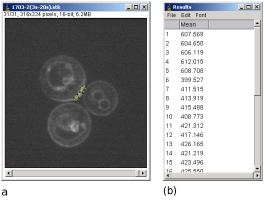
\includegraphics[width=3in]{ijmacrofig-frapresults.pdf}

 \caption{Measuring Stack Intensity Series. (a) Setting a Segmented ROI at the FRAPped area. (b) Results of Measuring Mean Intensity Dynamics.}

 \label{fig:frapresults}
\end{figure}

\begin{indentexercise}{1}
Modify code 10 to include more measurement parameters (whatever you like), and test the macro. Check the results. 

\item \textbf{Answer}:``Set Measurement'' could be added with more parameters to be measured, and the digits after the decimal point could be increased by increasing the number after ``decimal=''. For example, 
\begin{lstlisting}[numbers=none]
run("Set Measurements...", "area mean standard modal min centroid center perimeter bounding integrated median stack redirect=None decimal=5");
\end{lstlisting}

\end{indentexercise}

\begin{figure}[htbp]
\begin{center}
\includegraphics[scale=0.5]{fig/fig2322_moreResultsTable.png}
\caption{An example result after adding more measurement parameters.}
\label{fig_MoreMeasurementPara}
\end{center}
\end{figure} 


\subsection{Loop: while-looping}

Another way of letting a part of macro to loop is \textbf{while}-statement. In this case, iteration is not defined strictly. Looping continues until certain condition is met. As soon as the condition is violated, macro interpreter goes out from the loop.

\subsubsection{Basics of while statement}
Here is a simple example macro using \ilcom{while}.

\begin{lstlisting}[morekeywords={*, while}]
//Code 11
macro "while looping1" {
	counter=0;
	while (counter<=90) {
		print(counter);
		counter = counter + 10;
	}
}
\end{lstlisting}
\textbf{sourcecode}: \href{http://www.example.com/contents}{code/code11.ijm}
This macro prints out characters 0 to 90 with a 10 increment. 

\begin{figure}[htbp]
\begin{center}
\includegraphics[scale=0.4]{fig/fig2331_Code11out.png}
\caption{Output of code 11}
\label{fig:code11 output}
\end{center}
\end{figure} 

\begin{itemize}
\item line 3: The macro interpreter first assigns 0 to the counter.
\item line 4: The interpreter evaluates if the counter value is less than or equal to 90. Since counter is initially 0\ldots 
\item line 5: Printing function is executed. 
\item line 6: counter is added with 10. 
\item line 7: the interpreter realizes the end of "while" boundary and goes back to line 4. Since counter= 10 <= 90, line 5 is again executed\ldots and so on. When counter becomes 100 in line 6 after several more loops, counter is no longer <=90. So the interpreter goes out from the loop, moves to line 8. Then the macro is terminated.
\end{itemize}

Line 6 could be written in the following way as well.
\begin{lstlisting}[numbers=none]
counter += 10;
\end{lstlisting}
This means that "counter" is added with 10. Similarly, subtracting 10 from counter is 
\begin{lstlisting}[numbers=none]
counter -= 10;
\end{lstlisting}
Multiplication is 
\begin{lstlisting}[numbers=none]
counter *= 10;
\end{lstlisting}
Division is
\begin{lstlisting}[numbers=none]
counter /= 10;
\end{lstlisting}
If the increment is 1 or -1, (counter +=1 or counter-=1), then one could also write them  as 
\begin{lstlisting}[numbers=none]
counter++;
 or 
counter--;
\end{lstlisting}
These two last macro functions are said to work faster than +=1 or -=1, but I myself do not see much difference. Computers are fast enough these days. 

\begin{indentexercise}{1}
(1) Try changing code 11 so that it uses "+=" sign.\\
(2) Change code 11 so that it uses "++" sign, and prints out integers from 0 to 9.\\

\item \textbf{Answer}: (1) Change line 6 to \ilcom{counter += 1;}. (2) Change line 4 to \ilcom{while (counter<=9)} and line 6 to \ilcom{counter++}.
\end{indentexercise}

\begin{indentexercise}{2}
Change line 4 of code 11 to \ilcom{while (counter <0)} and check the effect (see below).
\end{indentexercise}

Evaluation of \ilcom{while} condition could also be at the end of loop. In this case, \ilcom{do} should be stated at the beginning of the loop. With do-while combination, the loop is always executed at least once, regardless of the condition defined by \ilcom{while} since macro interpreter reads lines from top to bottom. Write the following code.


\begin{lstlisting}[morekeywords={*, while}]
//Code 11.5
macro "while looping2" {
	counter=0;
	do {
		print(counter);
		counter += 10;
	} while (counter<0); 
}
\end{lstlisting}
\textbf{sourcecode}: \href{http://www.example.com/contents}{code/code11\_5.ijm}

In this example, the exit condition for going out from looping is \ilcom{counter < 0}, and the initial value of \ilcom{counter} is 0, which does not satisfy that looping condition. Since this evaluation occurs only after the looping part is executed for the first time, the macro still prints out a line before it exits from the loop.  


Condition for the while-statement could be various. Here is a small list of comparison operators.

\begin{indentCom}
 \begin{tabular*}{0.5\textwidth}{ l r }
< & less than \\
<= & less than or equal\\ 
> & greater than\\ 
>= & greater than or equal to\\
== & equal\\
!= & not equal\\
 \end{tabular*}
\end{indentCom}

\begin{indentexercise}{3}
Modify code 11 so that the macro prints out numbers from 200 to 100, with an increment of -10. 

\item \textbf{Answer}: There could be slightly various ways to do this modification, but here is one way. 
	\begin{lstlisting}
macro "while looping1" {
	counter=200;
	while (counter>=100) {
		print(counter);
		counter -= 10;
	}
}
\end{lstlisting}

\end{indentexercise}


\subsubsection{Why is there while-loop?}

An often raised question with the while-loop is why do we have two types of loops, 
the for-loop and the while-loop. Answering to this question, they have different
flexibility. The for-loop is rather solid and the while-loop is more flexible. In the
example code below, the user is asked for a correct number and if the answer is wrong, the
question is asked 5 times repeatedly. Number of loop is not determined by the
programmer, but interactively when the code is running. We will study
the branching of the program based on if-else in the next section.  


\begin{lstlisting}[morekeywords={*, while}]
macro "flexible loop by while" {
  answer_is_wrong = true;
  imagej_first_release = 1997;
  trial = 5;
  while (answer_is_wrong) {
    answer = getNumber("In which year did the first version of ImageJ released?", 1900);
    if (answer == imagej_first_release ){
      answer_is_wrong = false;
      showMessage("CORRECT! The year" + imagej_first_release);		
    } else {
      showMessage("NO. try again: trials left:" + trial);
      trial--;
    }
    if (trial < 1)
      answer_is_wrong = false;
  }
}
\end{lstlisting}
\textbf{sourcecode}: \href{http://www.example.com/contents}{code/code11\_6.ijm}

Writing a similar code using the for-loop is possible but the code becomes tricky.
Below is the for-loop version of the above code.  


\begin{lstlisting}[morekeywords={*, for}]
macro "flexible loop by for" {
  imagej_first_release = 1997;
  trial = 10;
  for (correct = 0; correct < 1; ) {
    answer = getNumber("In which year did the first version of ImageJ released?", 1900);
    if (answer == imagej_first_release ){
      showMessage("CORRECT! The year" + imagej_first_release);		
      correct++;
    } else {
      showMessage("NO. try again: trials left:" + trial);
      trial--;
    }
    if (trial < 1)
            correct++;
  }
}

\end{lstlisting}
\textbf{sourcecode}: \href{http://www.example.com/contents}{code/code11\_7.ijm}

Note that the third argument of for-loop is missing. Since the variable
\ilcom{correct} does not change as long as the answer is wrong, we leave it not
incrementing nor decrementing. In such case we can leave the third argument
vacant. 

\subsection{Conditions: if-else statements}
\subsubsection{Introducing if-else}
A macro program could have parts which are executed depending on some
conditions.
Here is an example of macro with conditions.

\begin{lstlisting}[morekeywords={*, if}]
//Code 12
macro "Condition_if_else 1"{
	input_num = getNumber("Input a number", 5);
	if (input_num == 5) {
		print(input_num+ ": The number is 5 ");
	} 
}
\end{lstlisting}
\textbf{sourcecode}: \href{http://www.example.com/contents}{code/code12.ijm}
\begin{itemize}
\item Line 3 The macro asks user to input a number and the number is substituted to the variable input\_num.
\item Line 4 Content of input\_num is evaluated. If input\_num is equal to 5, line 5 is executed and prints out the message in the Log window. Otherwise macro interpreter jumps to line 7, and ends the operation.  By adding "else" which will be executed if input\_num is not 5, the macro prints out message in all cases (see code 12.5 for this if - else case). 
\item Line 4 We used double equal signs for evaluating the value in the right side and the left side (e.g. \ilcom{if (a==5)}). 
Note that the role of the sign \ilcom{=} is different from assignments, or substitution (e.g. \ilcom{a = b + c}).
\end{itemize}
\begin{figure}[htbp]
\begin{center}
\includegraphics[scale=0.6]{fig/fig2341_code12out.png}
\caption{Output of code 12}
\label{fig:code12 output}
\end{center}
\end{figure} 

Now, we examine the content between 
parenthesis after ``if'' in more detail. 
Write the following code in your script editor and run it.

\begin{lstlisting}[morekeywords={*, ==}]
a = (5==5);
print(a);

\end{lstlisting}
\textbf{sourcecode}: \href{http://www.example.com/contents}{code/code12\_1.ijm}
The output in the log window should be \textit{1} indicating that ``\ilcom{(5 ==
5)}'' is \textit{1}. Next, modify the code like below and run it.

\begin{lstlisting}[morekeywords={*, ==}]
a = (5 == 4);
print(a);

\end{lstlisting}
\textbf{sourcecode}: \href{http://www.example.com/contents}{code/code12\_2.ijm}
The output is now 0, indicating that ``\ilcom{(5 == 4)}'' is
0.
What double equal signs \ilcom{==} are doing in these
examples are comparison of numbers in the left and the right side, and if
the numbers are the same, it returns 1 and if they are not the same, it returns 0. 1 and
0 actually are representing \textbf{true} (= 1) or \textbf{false} (= 0), the
\textbf{boolean values}.

We could also test if they are NOT equal. For this, replace \ilcom{==} by
\ilcom{!=}.

\begin{lstlisting}[morekeywords={*, !=}]
a = (5 != 4);
print(a);

\end{lstlisting}
\textbf{sourcecode}: \href{http://www.example.com/contents}{code/code12\_3.ijm}
Run the code above, and it returns 1, because 5 is NOT 4 and that is true. Now,
you could introduce the \textit{if} again as follows.

\begin{lstlisting}[morekeywords={*, if, else}]
if (5 != 4){
  print("true");
} 
  



\end{lstlisting}
\textbf{sourcecode}: \href{http://www.example.com/contents}{code/code12\_35.ijm}
In the parenthesis after ``if'', there is obvious TRUE statement (5 is not 4).
This is true, so the macro function bounded by curly braces is executed, which is to
print out ``true'' in the log window.

Try changing the line 2 to \ilcom{if (5 == 4)}. Running this prints nothing
in the log window, because 5 is not 4 (FALSE!) so that the macro function in
line 3 is ignored. To avoid such ignorant no-output behavior, you could add
``else'' as follows.


\begin{lstlisting}[morekeywords={*, if, else}]
if (5 == 4){
  print("true");
} else {
  print("false!");
}
  



\end{lstlisting}
\textbf{sourcecode}: \href{http://www.example.com/contents}{code/code12\_4.ijm}

The code works also with the direct true or false
declaration inside the if parenthesis. Try the following code.


\begin{lstlisting}[morekeywords={*, if, else}]
if (0){
  print("true");
} else {
  print("false!");
}

if (false){
  print("true");
} else {
  print("false!");
}

\end{lstlisting}
\textbf{sourcecode}: \href{http://www.example.com/contents}{code/code12\_5.ijm}

The above prints two lines of ``false!'' in the log window. You could replace
the if parenthesis values to 1 and true to check that it works as well. 

By now, it is probably pretty clear to you wi what is going on in the code below. 

\begin{lstlisting}[morekeywords={*, if, else}]
macro "Condition_if_else 2"{
	input_num = getNumber("Input a number", 5);
	if (input_num == 5) {
		print(input_num+ ": The number is 5 ");
	} else {
		print(input_num+ ": The number is not 5 ");
	}
	print("--------------");
}

\end{lstlisting}
\textbf{sourcecode}: \href{http://www.example.com/contents}{code/code12\_6.ijm}

\subsubsection{Complex Conditions}
In many cases, you might need to evaluate the condition of multiple variables at once. 
For such demands, several different comparisons can be combined by using following Boolean operators. 

\begin{indentCom}
 \begin{tabular*}{0.5\textwidth}{ l l }
\&\& & boolean AND\\
|| & boolean OR\\
\end{tabular*}
\end{indentCom}

Let's first test what these symbols do by directly using
\ilcom{true} and \ilcom{false} in macro.

\begin{lstlisting}[morekeywords={*, if, else}]
a = true;
b = true;
if (a && b){
  print("&& both true")
}

if (a || b){
  print("|| one of them or both is true")
}

\end{lstlisting}
\textbf{sourcecode}: \href{http://www.example.com/contents}{code/code12\_65.ijm}
When you run this code as it is, line 4 and line 8 are both executed and prints
the messages. For the first \ilcom{if} parenthesis, \ilcom{\&\&} operator tests if
both sides are true. If both are indeed true, it returns true (1), and that is
the case above. If one of them or both are false, then \ilcom{\&\&}
operator returns false(0). 

On the other hand, in the second if parenthesis,
\ilcom{||} operator tests if one of the two sides is true. Since both are
true in the above code, OR operator returns true because at least one of them is
true. Only when both sides are false, the returned value becomes false (0).

\begin{indentexercise}{1}
Adjust the values of \ilcom{a} and \ilcom{b} in code 12\_65 to \ilcom{true} or \ilcom{false} and
compose other three possible combinations (e.g. \ilcom{a = true}, \ilcom{b = false} will print
only one line). Check the output.

Next, change the values of \ilcom{a} and \ilcom{b} to 0 and/or
1 and check the results. 
\end{indentexercise}

Here is a more realistic example (though not very useful), an extended version
of code 16\_6.

\begin{lstlisting}[morekeywords={*, if, else}]
//Code 12.75------------------------------

macro "Condition_if_else 3"{
  input_num1 = getNumber("Input a number 1", 5);
  input_num2 = getNumber("Input a number 2", 6);
  message0 = ""+input_num1 + ","+input_num2;	//use this string four times
  if ( (input_num1==5) && (input_num2==6) ) {
    print(message0+ ": The parameter1 is 5 and the parameter2 is 6");
  } else {
    if (input_num1!=5) && (input_num2!=6) {
      print(message0 + ": The parameter1 is not 5 and the parameter2 is not 6");
    } else {
      if (input_num2==6) {
        print(message0 + ": The parameter1 is NOT 5 but the parameter2 is 6");
      } else {
        print(message0 + ": The parameter1 is 5 but the parameter2 is NOT 6");
      }
    }
  }
}
\end{lstlisting}
\textbf{sourcecode}: \href{http://www.example.com/contents}{code/code12\_75.ijm}
\begin{itemize}
\item Line 4 and 5 ask user to input two parameters.
\item Line 6 is for setting a string variable, to abbreviate a long string assignment that appears four times in the macro.
\item Line 7 evaluates these input parameters by comparing each of them separately, but the decision is made by associating two decisions with \ilcom{\&\&}. 
\item Line 10, != compares left and right sides of the operators and returns true if they are NOT equal.   
\end{itemize}
From line 10 to 17, there are several layers of conditions. Macro programmer should use tab-shifting for deeper condition layers as above for the visibility of code. Easy-to-understand code helps the programmer oneself to debug afterward, and also for other programmers who might reuse the code.
 		
\subsubsection{Application of if-statement}
\label{sec:dotmove}

As an application of looping and conditions, we write a macro that produces an animation of moving dot. User inputs the speed of the dot, and then the animation is generated. 
In the animation (which actually is a stack) the dot moves horizontally and bounces back from the edge
of the frame. 
\ilcom(if) operator is used to switch the movement direction.

\begin{lstlisting}[morekeywords={*, setForegroundColor, setBackgroundColor, if}]
//Code 13
macro "Generate Dot Animation back and forth" {

// **** initial values ****
	sizenum=10;	//dot size in pixel
	int=255;	//dot intensity in 8bit grayscale
	frames=50;	//frames in stack
	w=200;		//width of frame 
	h=50;		//height of frame 
	x_position = sizenum;	//starting x position: 
	y_position= (h/2)-(sizenum/2);	//y positon of the oval top-left corner: constant

//**** set colors *****
	setForegroundColor(int, int, int);
	setBackgroundColor(0, 0, 0);

//**** ask speed *****
	speed=getNumber("Speed [pix/frame]?",10)

//**** prepare stack ****
	stackname="dotanimation"+speed;	
	newImage(stackname, "8-bit Black", w, h, frames);

//**** drawing oval in the stack ****
	for(i=0; i<frames; i++) {
		setSlice(i+1);
		x_position += speed;
		if ((x_position > (w-sizenum)) || (x_position < 0) ) { 
			speed*=-1;
			x_position += speed*2;  //avoids penetrating boundary
		}
		makeOval(x_position, y_position, sizenum, sizenum);
		run("Fill", "slice");
	}
	run("Select None");
}

\end{lstlisting}
\textbf{sourcecode}: \href{http://www.example.com/contents}{code/code13.ijm}

\begin{itemize}
\item Lines 4 to 11: Set parameters for drawing a dot. It is also possible to directly use numerical values in the later lines, but for the sake of readability of the code, and also for possible later extension of the code, it is always better to use easy-to-understand variable names and explicitly define them before the main part starts. 
\item A short note on the x-y coordinate system in digital images: Since digital image is a matrix of numbers, each pixel position is represented as coordinates. The top left corner of image is the position (x, y) = (0, 0). X increases horizontally towards right side of the image. Y increases vertically towards the bottom of the image.  In line 11, y-position of the dot is defined to be placed in the middle of the vertical axis. 
\item Lines 14, 15: These lines set the drawing and background color. Three arguments are for intensity of each RGB component. Here the image is in grayscale so all the RGB components are set to the same value. 0 is black, and \ilcom{int} is white (255).
\item Line 18 asks the user to input the speed of the dot movement.
\item Lines 21, 22 prepares a new stack with parameters defined in lines 7, 8 and 9.
\item Lines 25 to 34 is the loop for drawing moving dot. Loop will be iterated from the starting frame until the last frame. Line 32 creates an oval Region-of-Interest (ROI), which will be filled in line 33 with the foreground color that was already set in the line 14. \ilcom{makeOval} function is explained in the Built-in function page as follows.

\begin{indentCom}
\textbf{makeOval}(x, y, width, height)\\
Creates an elliptical selection, where (x,y) defines the upper left corner of the bounding rectangle of the ellipse. 
\end{indentCom}
\item Line 27: Shifts the x position of the dot by ``speed'' distance. 
\item Line 28: if the position calculated in the line 27 exceeds the boundary, either left \ilcom{(x\_position < 0)} OR right \ilcom{(x\_position > (w-sizenum))}, then the direction of movement is switched by multiplying -1.
\end{itemize}
\begin{indentexercise}{2}
Modify code 13 that the dot moves up and down vertically. Change the stack width and height as well. 

If you are successful with this, try further on to extend the code so that the dot moves both in x and y directions. For this, you need to have two independent speed \ilcom{xspeed} and \ilcom{yspeed} since change in the direction by bouncing should be independent in x and y. 

\item \textbf{Answer}: By swapping x and y values, the movement becomes vertically oriented. We first swap the values of frame size and the initial position of the dot.  
	\begin{lstlisting}[numbers=none]
		w = 50;
		h = 200;
		x_positon =  (w/2)-(sizenum/2);
		y_position = sizenum;
	\end{lstlisting}
	Then line 27 to 31 should be changed to move the dot in y (vertical) direction, and also to change the condition for bouncing at walls.
	\begin{lstlisting}[numbers=none]
		y_position += speed;
		if ((y_position > (h-sizenum)) || (y_position < 0) ) { 
			speed*=-1;
			y_position += speed*2;
		}
	\end{lstlisting}

\end{indentexercise}

\end{document}
